\documentclass[compress]{beamer}
\usetheme{Warsaw}
\usecolortheme{wolverine}
\usefonttheme[onlylarge]{structurebold}
\setbeamerfont*{frametitle}{size=\normalsize,series=\bfseries}
\setbeamertemplate{navigation symbols}{}
\setbeamertemplate{footline}
{%
\begin{beamercolorbox}[wd=0.5\textwidth,ht=3ex,dp=1.5ex,leftskip=.5em,rightskip=.5em]{author
in head/foot}%
\usebeamerfont{author in head/foot}%
\hfill\insertshortauthor%
\end{beamercolorbox}%
\vspace*{-4.5ex}\hspace*{0.5\textwidth}%
\begin{beamercolorbox}[wd=0.5\textwidth,ht=3ex,dp=1.5ex,left,leftskip=.5em]{title
in head/foot}%
\usebeamerfont{title in head/foot}%
\insertshorttitle\hfill\insertframenumber/\inserttotalframenumber%
\end{beamercolorbox}%
}
\beamertemplatesolidbackgroundcolor{black!5}
\beamertemplatetransparentcovered

\usepackage[utf8]{inputenc}
\title{Das Freie Betriebsystem Linux}
\author{Frank Lanitz}
\date{\today}
\begin{document}
\frame{\titlepage}
\begin{frame}
	\tableofcontents{}
\end{frame}

\begin{frame}
	\frametitle{Vorstellungsrunde}
	\begin{block}{Über mich}
		\begin{itemize}
			\item Bis letzte Systembetreuer an der Universität Jena 
				\begin{itemize}
					\item Linux
					\item PostgreSQL
					\item ...
				\end{itemize}
			\item Jetzt: Administrator bei der Max-Planck-Gesellschaft
			\item Im Vorstand des Hackspace Jena e.V.
			\item Aktiv im Umfeld der FLOSS
			\item Mitarbeit bei Geany seit ca. 7 Jahren u.a. 
			\begin{itemize}
				\item Übersetzungen
				\item Maintainer verschiedener Plugins
				\item Mailingliste, IRC, \dots
			\end{itemize}
		\end{itemize}
	\end{block}
\end{frame}
\begin{frame}
	\frametitle{Das Publikum}
	\center{\Huge{Wer seit Ihr so?}}
\end{frame}

\section{Freie Software}
\subsection{Urheberrecht, Copyright \dots}
\begin{frame}
	\frametitle{Urheberrecht und Copyright}
	\begin{block}{Allgemein}
		\begin{itemize}
			\item Urheberrechte/Copyright wohnt allem Geschaffenen inne
			\item Allgemein gilt: Recht auf Festlegung, was mit einem Werk 
				passiert
			\item Auslegungsunterschiede je nach Rechtsraum
		\end{itemize}
	\end{block}
	\pause
	\begin{block}{Deutschland}
		\begin{itemize}
			\item Urheberrecht kann nicht abgegeben werden
			\item Software wird analog zu Sprachwerken behandelt (§ 69a Abs 4)
			\item Nutzer muss eine Lizenz zur Verwendung haben
		\end{itemize}
	\end{block}
	\pause
	\textbf{Aber: Ich bin kein Anwalt \dots}
\end{frame}

\subsection{Freie Software}
\begin{frame}
	\frametitle{Freie Software}
	\begin{block}{}
		\begin{itemize}
			\item Unterscheidung zwischen Freeware und freier 
				Software (free software)
			\item “Free as in ‘freedom’, not as in ‘free beer’”
				(Richard Stallman)
			\item Verschiedene Definitionen 
			\item Merkmale von Open Source
			\begin{enumerate}
				\item Quellcode liegt in lesbarer und verständlicher Form vor
				\item Quellcode darf beliebig oft kopiert, verbreitet und 
					genutzt werden
				\item Quellcode darf verändert und in der veränderten Form 
					weitergegeben werden
			\end{enumerate}
		\end{itemize}
	\end{block}
\end{frame}

\begin{frame}
	\frametitle{Finanzierung}
	\begin{block}{Prämisse}
		\begin{itemize}
			\item Das Problem steht vor der Lösung
		\end{itemize}
	\end{block}
	\pause
	\begin{block}{Finanzierung von FLOSS}
		\begin{itemize}
			\item Auftragsarbeiten: "Ich benötige ein Programm, um XYZ zu machen"
			\item Kommerzieller Support
			\item Spenden
			\item Merchandising 
		\end{itemize}
	\end{block}
	\pause
	$\rightarrow$ Datenkanal 002 (\url{http://yaturl.net/cdaa})
\end{frame}

\section{Betriebsystem}
\begin{frame}
	\frametitle{Betriebssystem}
	\begin{center}
	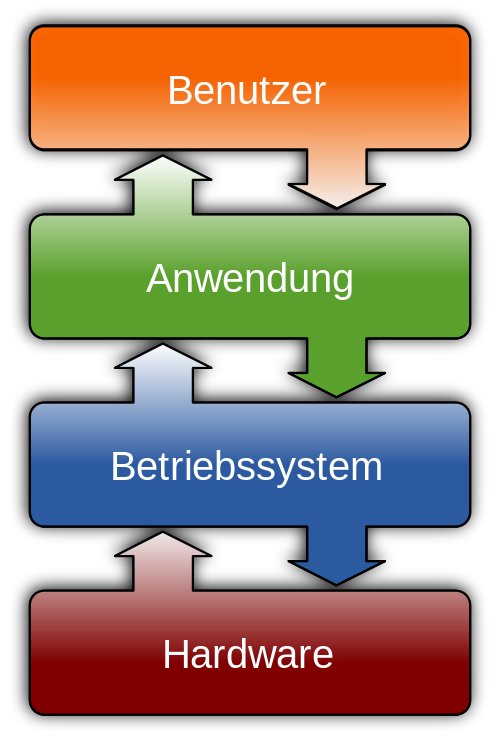
\includegraphics[scale=0.25]{media/500px-Operating_system_placement-de.png}
	\end{center}
	\raggedleft{\tiny aus der Wikipedia}
\end{frame}
\begin{frame}
	\begin{block}{}
		\begin{itemize}
			\item Viele verschiedene Systeme 
			\item Anwendungsspezifisch optimiert
				\begin{itemize}
					\item Echtzeit
					\item Minimalistisch
					\item General
					\item Desktop/Server
					\item Mobile Geräte 
				\end{itemize}
		\end{itemize}
	\end{block}
	\begin{block}{Beispiele}
		\begin{itemize}
			\item DOS - Disc Operating System
			\item Microsoft Windows
			\item Unixoide Systeme
				\begin{itemize}
					\item GNU/Linux
					\item *BSD: Open/Free/PC/Dragefly/Net
					\item AIX
					\item MacOS X
				\end{itemize}
		\end{itemize}
	\end{block}
\end{frame}

ssection{Linux}

\begin{frame}
	\frametitle{Nur der Kern}
\end{frame}

\begin{frame}
	\frametitle{Die Qual der Wahl - Distributionen wohin das Auge reicht}
	\begin{block}{}
		\begin{itemize}
			\item Für jedes Problem gibt es mindestens zwei Lösungen
		\end{itemize}
	\end{block}
\end{frame}

\begin{frame}
	\frametitle{Bezugsquellen von Linux}
	\begin{itemize}
		\item Download aus dem Internet
		\item Kauf eines Paketes bei z.B. MediaMarkt, Amazon, Thalia
		\item Vorinstalliert (z.B. Dell)
	\end{itemize}
\end{frame}

\begin{frame}
	\frametitle{Wo gibt es Hilfe}
	\begin{itemize}
		\item Handbücher, Fachbücher, Zeitschriften
		\item Internet: Newsgroups, Foren, Mailinglisten, IRC
		\item Kommerzeller Support
		\item Nette Leute, die gerne weiterhelfen (Linux User Group, Freunde \& Bekannte)
	\end{itemize}
\end{frame}



\end{document}
